\documentclass[10pt,twocolumn,letterpaper]{article}
\usepackage[margin=0.72in,columnsep=0.24in,top=0.8in,bottom=0.85in]{geometry}
\usepackage{newtxtext,newtxmath}
\usepackage[T1]{fontenc}
\usepackage{microtype}
\usepackage{graphicx}
\usepackage{booktabs}
\usepackage{multirow}
\usepackage{amsmath}
\usepackage{bm}
\usepackage[numbers,sort&compress]{natbib}
\usepackage[font=small,labelfont=bf,skip=4pt]{caption}
\usepackage{xcolor}
\usepackage{tikz}
\usetikzlibrary{arrows.meta,positioning,fit,backgrounds,calc}
\usepackage{enumitem}
\setlist{nosep,leftmargin=*,topsep=2pt}
\usepackage{titlesec}
\usepackage{fancyhdr}
\usepackage{placeins}
\definecolor{accent}{HTML}{1F4E8C}
\definecolor{inkgrey}{HTML}{52514E}
\definecolor{blk}{HTML}{2A78D6}
\definecolor{org}{HTML}{EB6834}
\definecolor{grn}{HTML}{1BAF7A}
\usepackage[colorlinks=true,linkcolor=accent,citecolor=accent,urlcolor=accent]{hyperref}
\usepackage[capitalise,noabbrev]{cleveref}

\titleformat{\section}{\large\bfseries\color{accent}}{\thesection}{0.6em}{}
\titleformat{\subsection}{\normalsize\bfseries}{\thesubsection}{0.5em}{}
\titleformat{\paragraph}[runin]{\normalsize\bfseries}{}{}{}[.]
\titlespacing*{\section}{0pt}{8pt}{3pt}
\titlespacing*{\subsection}{0pt}{5pt}{2pt}
\titlespacing*{\paragraph}{0pt}{3pt}{0.6em}
\setlength{\emergencystretch}{1.5em}

\pagestyle{fancy}
\fancyhf{}
\renewcommand{\headrulewidth}{0pt}
\fancyfoot[C]{\small\color{inkgrey}\thepage}
\fancyhead[R]{\small\color{inkgrey}\itshape Graded robustness and residual RL for a small VLA}
\fancypagestyle{plain}{\fancyhf{}\fancyfoot[C]{\small\color{inkgrey}\thepage}}

% generated by scripts/make_figures.py from results/ -- do not edit by hand
\newcommand{\BaseGoal}{20/20 (100\%, CI 84--100)}
\newcommand{\BaseGoalPct}{100\%}
\newcommand{\BaseSpatial}{59/100 (59\%, CI 49--68)}
\newcommand{\BaseSpatialPct}{59\%}
\newcommand{\CamXfifty}{30}
\newcommand{\CamXfiftyCI}{[22, 40]}
\newcommand{\CamXfiftyInterp}{>30}
\newcommand{\CamXfiftyInterpCI}{[15, >30]}
\newcommand{\EvalCheckP}{0.74}
\newcommand{\LangAbsurd}{0/50}
\newcommand{\LangDiag}{25/30 (83\%, CI 66--93)}
\newcommand{\LangEmpty}{0/50}
\newcommand{\LangOffEnv}{0\%}
\newcommand{\LangOffEnvFrac}{0/270}
\newcommand{\LangOffInstructed}{73\%}
\newcommand{\LangOffInstructedFrac}{197/270 (73\%, CI 67--78)}
\newcommand{\LangOther}{2/270}
\newcommand{\LangPara}{35/150 (23\%, CI 17--31)}
\newcommand{\LangParaClose}{20/50}
\newcommand{\LangParaDistant}{4/50}
\newcommand{\LangParaReworded}{11/50}
\newcommand{\LangVariantsFailed}{215}
\newcommand{\LangVariantsFailedAnyGoal}{0}
\newcommand{\LerobotEvalCheck}{14/20 (70\%)}
\newcommand{\LightCliffHigh}{81\%}
\newcommand{\LightCliffLow}{67.5\%}
\newcommand{\LightXfifty}{0.76}
\newcommand{\LightXfiftyCI}{[0.72, 0.81]}
\newcommand{\LightXfiftyInterp}{0.74}
\newcommand{\LightXfiftyInterpCI}{[0.72, 0.78]}
\newcommand{\OurEvalCheck}{12/20 (60\%)}
\newcommand{\RLCleanRes}{8/10}
\newcommand{\RLCleanResPct}{80\%}
\newcommand{\RLCleanVla}{8/10}
\newcommand{\RLCleanVlaPct}{80\%}
\newcommand{\RLSeeds}{1}
\newcommand{\RLStrongRes}{1/10}
\newcommand{\RLStrongResPct}{10\%}
\newcommand{\RLStrongVla}{1/10}
\newcommand{\RLStrongVlaPct}{10\%}
\newcommand{\RLTrainRes}{4/10}
\newcommand{\RLTrainResPct}{40\%}
\newcommand{\RLTrainVla}{5/10}
\newcommand{\RLTrainVlaPct}{50\%}
\newcommand{\RobotXfifty}{0.078}
\newcommand{\RobotXfiftyCI}{[0.05, 0.11]}
\newcommand{\RobotXfiftyInterp}{0.048}
\newcommand{\RobotXfiftyInterpCI}{[0.031, 0.082]}
\newcommand{\TotalEpisodes}{1\,755}

% generated by scripts/make_tables.py
\newcommand{\AllEpisodes}{3\,335}
\newcommand{\EvalHours}{24}
\newcommand{\PPOHours}{10}
\newcommand{\TotalHours}{34}
\newcommand{\NSeeds}{3}
\newcommand{\SeedsWord}{three}

% text that depends on the random-sign residual runs (filled in once they finish)
\newcommand{\RLRandAbstract}{even when trained on more diverse starting poses, and mostly learns to finish successful episodes faster.}
\newcommand{\RLRandConclusion}{A residual corrector trained on a few hundred episodes does not repair the arm-pose weakness on unseen configurations, and more diverse arm offsets during training do not change this; generalising likely requires more varied scenes or an input that encodes the scene, not only proprioception.}

\begin{document}

\twocolumn[{%
\begin{center}
  {\LARGE\bfseries Does a Small VLA Listen, and Where Does It Break?\par}
  \vspace{4pt}
  {\large Graded robustness of SmolVLA on LIBERO, and a residual RL correction\par}
  \vspace{10pt}
  {\normalsize Ana\"is Azouaoui\par}
  \vspace{1pt}
  {\small\color{inkgrey} Sorbonne Universit\'e, Paris, France \quad\textbullet\quad
  \href{https://github.com/ananalab/vla-stress-test}{\texttt{github.com/ananalab/vla-stress-test}}\par}
  \vspace{10pt}
  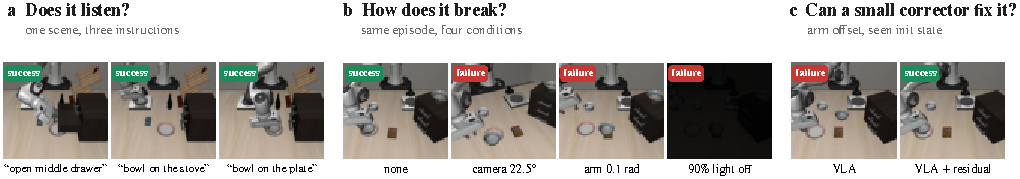
\includegraphics[width=\textwidth]{figures/teaser.pdf}
  \captionof{figure}{\textbf{Three questions about a small vision-language-action model.}
  (a)~In one LIBERO-Goal scene, the same policy carries out whichever instruction it is given.
  (b)~The same episode fails under a camera rotation, a few degrees of arm offset at the start, or dim light.
  (c)~A residual policy trained by PPO on top of the frozen model can rescue episodes it was trained on.
  All frames are the model's own camera input.}
  \label{fig:teaser}
  \vspace{8pt}
\end{center}
}]

\begin{abstract}
\noindent Vision-language-action (VLA) models are almost always evaluated in the conditions they were
trained on. We study SmolVLA~\citep{shukor2025smolvla}, a 450M-parameter open VLA, on the LIBERO
benchmark~\citep{liu2023libero} through three questions. \emph{Does it listen?} In LIBERO-Goal, where ten
tasks share one scene, we swap instructions and evaluate all ten goal predicates at every step: the
robot reaches the goal of the instruction it is given in \LangOffInstructed{} of swapped episodes and the
environment's own goal in \LangOffEnv{}, yet paraphrases of an instruction succeed far less often than its
original wording (\LangParaPct{} against \LangOrigPct{}). Mapping each instruction to the closest training
instruction with a sentence encoder restores the original level on LIBERO-Goal, and only partly on
LIBERO-Spatial, whose instructions differ by a spatial relation. \emph{How does it break?} Swept over a
continuous intensity, success declines gradually with camera viewpoint, collapses past sharp thresholds
for lighting and pixel noise, and is halved by about $3^\circ$ of offset per arm joint at the start of
the episode. A MAP-Elites search over combinations of four perturbations, each harmless on its own,
finds failures almost everywhere: the most harmful combinations make \QDValPooledPct{} of held-out
episodes fail, and in \QDPurePct{} of them every component alone, at the same value, succeeds. \emph{Can a small corrector help?} A residual
policy trained with PPO on top of the frozen model improves success on the initial states it was trained
on but not on held-out ones, \RLRandAbstract{} The study comprises \AllEpisodes{} simulated episodes and
about \TotalHours{} hours of compute on a laptop; all per-episode logs, code and figure scripts are
released.
\end{abstract}

% =====================================================================================
\section{Introduction}
VLA models map a camera image and a sentence to robot actions with a single network built on a
pretrained vision-language model. On simulation benchmarks such as LIBERO their success rates approach
saturation, which says little about two questions that matter once the robot leaves the benchmark: is
the instruction actually used, and how does performance degrade when the scene departs from the
demonstrations? Recent robustness suites~\citep{fei2025liberoplus,zhou2025liberopro} address the second
question with many perturbation types at a few fixed levels and conclude that VLAs are fragile to
viewpoint and initial state and largely ignore language.

We take a narrower and more quantitative look at a single small model, SmolVLA, chosen because it is open,
fits on consumer hardware and is integrated in LeRobot~\citep{cadene2024lerobot}. Our contributions are:
\begin{itemize}
  \item A \textbf{goal-level listening test}. Because all LIBERO-Goal tasks share the same objects, we
  can evaluate every task's goal at every step. This separates a robot that ignores the instruction from
  one that follows it but fails, which success on the environment's own goal cannot do.
  \item An \textbf{input-side repair} of the paraphrase brittleness: retrieval of the closest training
  instruction, with a rejection threshold so that unrelated requests are not turned into tasks.
  \item \textbf{Dose-response curves} for five perturbations with a continuous intensity, a breaking
  point $x_{50}$ estimated in two ways with task-level bootstrap intervals, and per-task curves.
  \item A \textbf{search for interaction failures}: MAP-Elites~\citep{mouret2015mapelites} over combinations of
  perturbations that are each harmless on the episodes used, validated on held-out episodes.
  \item A \textbf{residual RL} experiment targeting the weakness that is visible in proprioception, with
  an evaluation on held-out initial states that distinguishes learning from generalising.
  \item A \textbf{validated, reproducible pipeline}: a cross-check against the official evaluation,
  episode-level determinism checks, tests that each perturbation changes the policy input, and a paired
  design in which every condition is evaluated on the same episodes.
\end{itemize}

% =====================================================================================
\section{Related work}
\paragraph{Vision-language-action models} OpenVLA, $\pi_0$ and related models fine-tune large
vision-language backbones to output actions; SmolVLA~\citep{shukor2025smolvla} reduces the backbone to a
truncated 500M SmolVLM2 and adds a flow-matching~\citep{lipmanflow2022} action expert that predicts chunks
of 50 actions, reaching performance comparable to much larger models on LIBERO.

\paragraph{Robustness of VLAs} LIBERO-Plus~\citep{fei2025liberoplus} perturbs LIBERO along seven axes
(camera, robot initial state, language, lighting, background, sensor noise, layout) and reports that
camera and initial-state changes are the most damaging while language variations matter little, which the
authors interpret as models ignoring language. LIBERO-PRO~\citep{zhou2025liberopro} shows that success can
collapse under object, position and instruction changes and attributes high scores to memorisation. We
reuse their axes but sweep intensity continuously, and replace success on the environment's goal by an
evaluation of all goals of the shared scene.

\paragraph{Search-based testing of learned systems} Vision-based driving controllers have been tested
by evolutionary search over scenario parameters~\citep{abdessalem2018testing}, and Quality-Diversity
search has been used to map the feature space of deep-learning systems where they
misbehave~\citep{zohdinasab2021deephyperion} or the frontier between correct and incorrect
behaviour~\citep{riccio2020deepjanus}. We use MAP-Elites in the same spirit, restricted to perturbations that
are harmless one at a time, so that every failure found is an interaction.

\paragraph{Residual policy learning} Residual RL learns an additive correction on top of a fixed
controller~\citep{silver2018residual,johannink2019residual}. ResiP~\citep{ankile2024resip} and Policy
Decorator~\citep{yuan2024policydecorator} refine imitation-learned diffusion or transformer policies this
way, with a correction bounded in magnitude and initialised to zero. We apply the same recipe to a VLA,
targeting one specific robustness failure.

% =====================================================================================
\section{Experimental setup}


\begin{figure}[t]
\centering
\resizebox{\columnwidth}{!}{%
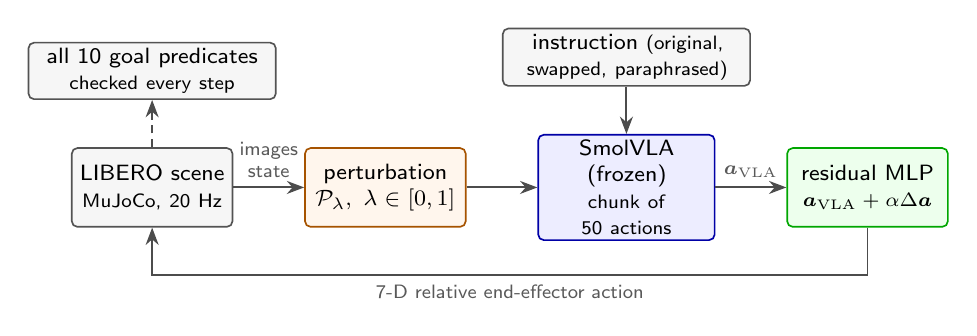
\begin{tikzpicture}[
  font=\sffamily\footnotesize,
  box/.style={draw=#1!65!black, fill=#1!7, rounded corners=2pt, minimum height=10mm, text width=19mm, align=center, inner sep=2pt, line width=0.6pt},
  arr/.style={-{Stealth[length=2.2mm]}, line width=0.7pt, color=black!70},
  lab/.style={font=\sffamily\scriptsize, color=black!65, align=center}]
  \node[box=gray] (sim) {LIBERO scene\\{\scriptsize MuJoCo, 20 Hz}};
  \node[box=orange, right=9mm of sim] (pert) {perturbation\\$\mathcal{P}_\lambda,\ \lambda\in[0,1]$};
  \node[box=blue, right=9mm of pert, text width=21mm] (vla) {SmolVLA (frozen)\\{\scriptsize chunk of 50 actions}};
  \node[box=green, right=9mm of vla] (res) {residual MLP\\{\scriptsize $\bm a_\mathrm{VLA}+\alpha\Delta\bm a$}};
  \node[box=gray, above=6mm of vla, text width=30mm, minimum height=7mm] (instr) {instruction {\scriptsize(original, swapped, paraphrased)}};
  \node[box=gray, above=6mm of sim, text width=30mm, minimum height=7mm] (goal) {all 10 goal predicates {\scriptsize checked every step}};
  \draw[arr] (sim) -- node[lab, above] {images\\state} (pert);
  \draw[arr] (pert) -- (vla);
  \draw[arr] (instr) -- (vla);
  \draw[arr] (vla) -- node[lab, above] {$\bm a_\mathrm{VLA}$} (res);
  \draw[arr, densely dashed] (sim) -- (goal);
  \draw[arr] (res.south) -- ++(0,-6mm) -| node[lab, pos=0.25, below] {7-D relative end-effector action} (sim.south);
\end{tikzpicture}}
\caption{\textbf{Evaluation loop.} Perturbations act on the simulator after each reset (camera, lights,
arm pose) or on the images given to the policy (noise, masking); the instruction is replaced for the
language tests. The residual corrector is only used in \cref{sec:rl}; elsewhere $\bm a=\bm a_\mathrm{VLA}$.}
\label{fig:pipeline}
\end{figure}

\subsection{Model, simulator and evaluation loop}
We use the Hub checkpoint \texttt{lerobot/smolvla\_libero} (revision \texttt{31d453f}), fine-tuned on the
LIBERO demonstrations with LeRobot. The policy receives the third-person (\emph{agentview}) and wrist images at
$360\times360$, an 8-D state (end-effector position, axis-angle orientation, gripper opening) and the
instruction, and outputs a chunk of 50 relative end-effector actions sampled with 10 flow-matching steps;
the whole chunk is executed before the next query, as in the checkpoint's configuration. Observations go
through the pre- and post-processors saved with the checkpoint (normalisation, tokenisation, camera renaming),
so the model sees exactly what it would see under \texttt{lerobot-eval}. Episodes end on success or after
280 (Spatial) or 300 (Goal) steps.

Everything ran on an Apple M1 laptop with 8\,GB of memory: LIBERO runs natively on macOS with offscreen
CGL rendering once an unused Linux-only dependency is skipped, and the policy runs on the Metal backend
with the checkpoint's bf16 weights (\cref{tab:compute}). We use LIBERO-Spatial for perturbations (ten
tasks with distinct layouts) and LIBERO-Goal for language (ten tasks in one scene).

\subsection{Protocol}
Episode $e$ of a task always starts from LIBERO's $e$-th fixed initial state with random seed $e$, which also
fixes the flow-matching noise, whatever the condition. Two conditions therefore differ only by the
perturbation, and outcomes can be compared episode by episode. Every episode uses a hard reset (the MuJoCo
model is rebuilt), and each row of the result files records configuration, seed, commit, library versions,
checkpoint revision and device. Baseline and language experiments use 10 and 3--5 episodes per task;
dose-response experiments use 5 episodes per task and level (50 per level).

\begin{figure*}[t]
  \centering
  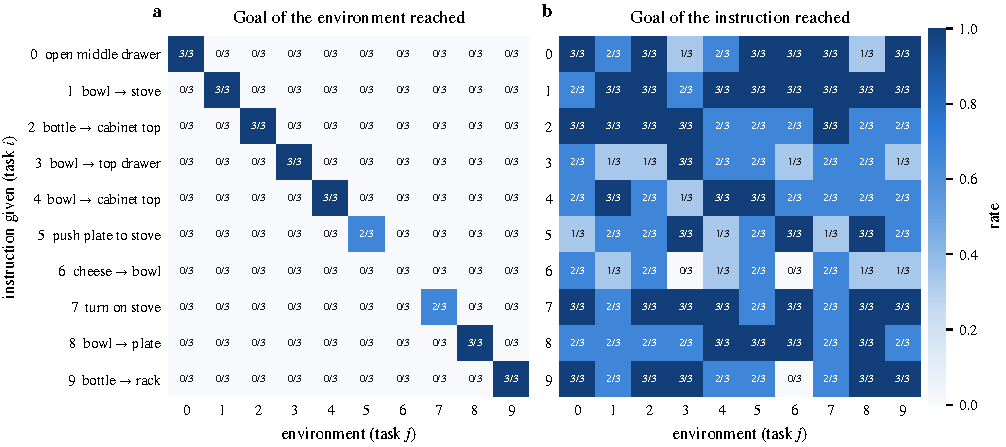
\includegraphics[width=\textwidth]{figures/language_matrix.pdf}
  \caption{\textbf{Listening test} (3 episodes per cell, 300 episodes). The environment of task $j$ is
  built and the instruction of task $i$ is given. (a)~Goal $j$ reached, as scored by the environment.
  (b)~Goal of the \emph{given} instruction $i$ reached at any step. Off the diagonal, the robot never
  completes the environment's task but completes the instructed one in \LangOffInstructedFrac{} of episodes.}
  \label{fig:language}
\end{figure*}

\subsection{Statistics}
Success rates are reported with Wilson 95\% intervals~\citep{wilson1927}, which stay inside $[0,1]$ and
behave well for small $n$ and extreme rates. Paired conditions are compared with an exact McNemar test on
discordant episodes. For a perturbation of intensity $x$ (in physical units) we fit
\begin{equation}
  p(x) = \frac{s_0}{1+\exp\!\big((x-x_{50})/w\big)}
  \label{eq:logistic}
\end{equation}
by binomial maximum likelihood with $s_0$ fixed to the unperturbed success rate on the same episodes, so
that $x_{50}$ is the intensity at which success is halved. Because a logistic cannot represent every shape
(a plateau followed by a cliff and a long tail, for instance), we also report a model-free $x_{50}$: pooled
success per level is made non-increasing by isotonic regression and linearly interpolated at $s_0/2$.
Intervals on both estimates come from a bootstrap over \emph{tasks} (300 resamples of whole tasks), since task difficulty varies far more than outcomes within a task.

\subsection{Validating the pipeline}
\label{sec:validation}
\paragraph{Official evaluation} On two LIBERO-Spatial tasks the official \texttt{lerobot-eval} gives
\LerobotEvalCheck{} and our loop \OurEvalCheck{} (Fisher $p=\EvalCheckP$).
\paragraph{Determinism} Re-running recorded episodes reproduces their outcome \emph{and} their exact
length, on the Metal backend and after rebuilding the Python environment from scratch.
\paragraph{Perturbations reach the policy} Unit tests check that each perturbation changes the policy's
input image, monotonically with intensity, and is the identity at intensity 0. The first version of the
camera and lighting perturbations silently did nothing: camera poses are only recomputed by MuJoCo's
forward pass, and robosuite caches observations between simulation steps. Without the image check the
dose-response curves would have been flat for the wrong reason. For language, we decode the token
sequence actually passed to the model.

\begin{table}[t]
\centering
\caption{\textbf{Unperturbed success.} Wilson 95\% intervals in brackets. The reported numbers may refer to
a different checkpoint than the one on the Hub.}
\label{tab:baselines}
\small
\resizebox{\columnwidth}{!}{% generated by scripts/make_tables.py -- do not edit
\begin{tabular}{lcc}
\toprule
Suite & This work (10 tasks $\times$ 10) & Reported~\citep{shukor2025smolvla} \\
\midrule
LIBERO-Spatial & 59/100 (59\%) [49, 68] & 90\% \\
LIBERO-Goal & 84/100 (84\%) [76, 90] & 92\% \\
\midrule
\multicolumn{3}{l}{\footnotesize Cross-check on Spatial tasks 1 and 3: \texttt{lerobot-eval} 14/20, this loop 12/20.} \\
\bottomrule
\end{tabular}
}
\end{table}

\paragraph{Baselines} \Cref{tab:baselines} gives \BaseSpatial{} on LIBERO-Spatial and \BaseGoal{} on
LIBERO-Goal, below the 90\% and 92\% reported in~\citep{shukor2025smolvla}. The cross-check above rules
out our loop as the cause; the Hub checkpoint was trained separately from the paper's runs. All conclusions
below are relative to the measured baseline, and tasks vary widely (\cref{tab:pertask}).

% =====================================================================================
\section{Does the model listen?}
\label{sec:language}
\subsection{Swapping instructions in a shared scene}


All ten LIBERO-Goal tasks are defined on the same objects (a bowl, a plate, a bottle, a cream cheese box, a
stove, a cabinet with drawers, a rack) and differ only by their instruction, goal predicate and set of
initial states. We build the environment of task $j$, which scores goal $j$, give the instruction of task
$i$, and in addition evaluate the ten goal predicates at every step. $M_{ij}$ is either the rate at which
goal $j$ is reached (what the environment reports) or the rate at which the instructed goal $i$ is reached.



Read alone, \cref{fig:language}a is ambiguous: success only on the diagonal is what a robot that ignores
language would also produce if its default behaviour did not happen to satisfy goal $j$.
\Cref{fig:language}b resolves it. Told to do task $i$ in the scene of task $j$, the robot reaches goal $i$
in \LangOffInstructed{} of the 270 swapped episodes, close to the rate with matched instructions
(\LangDiag{}), never reaches the environment's goal (\LangOffEnvFrac{}), and completes a third, unrelated
goal in only \LangOther{} episodes. The initial states of the ten tasks differ slightly, so the behaviour is
not keyed on the starting configuration either. Instructions involving cluttered targets are followed less
reliably (task 3, bowl into the top drawer; task 6, cream cheese into the bowl). \Cref{fig:teaser}a shows one scene
under three instructions.



\begin{figure*}[t]
  \centering
  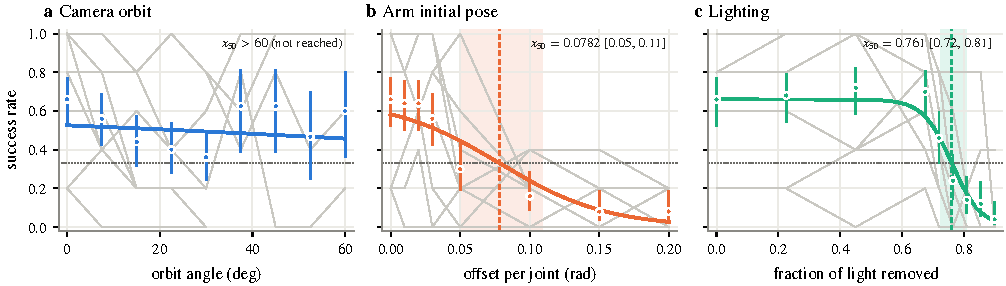
\includegraphics[width=\textwidth]{figures/dose_response.pdf}\\[2pt]
  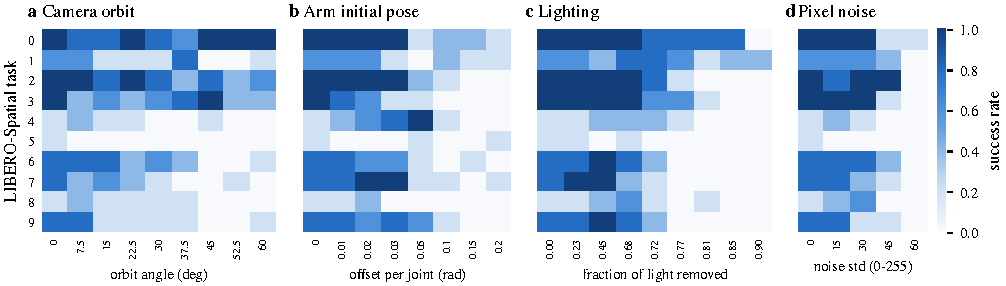
\includegraphics[width=\textwidth]{figures/dose_per_task.pdf}
  \caption{\textbf{Success versus perturbation intensity} on LIBERO-Spatial (10 tasks $\times$ 5 episodes per
  level; the unperturbed point uses the same episodes). \emph{Top:} pooled success with Wilson 95\% intervals,
  individual tasks in grey, logistic fit (\cref{eq:logistic}) with half the baseline dotted, and logistic
  $x_{50}$ with its 95\% task-bootstrap interval (dashed line and band). \emph{Bottom:} success per task and
  level (5 episodes per cell), same levels as the top row.}
  \label{fig:dose}
\end{figure*}

\subsection{\dots{} but to the exact words}
\begin{figure}[t]
  \centering
  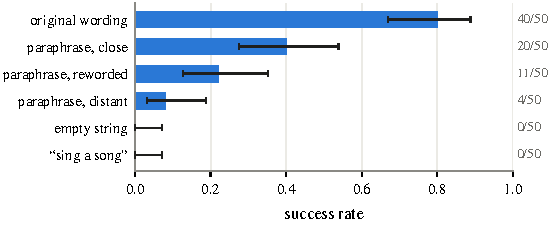
\includegraphics[width=\columnwidth]{figures/language_variants.pdf}
  \caption{\textbf{Instruction variants} on LIBERO-Goal (environment and instruction of the same task, 5
  episodes per task and variant). Paraphrases were written by hand and are listed in \texttt{configs/language\_variants.yaml}.}
  \label{fig:variants}
\end{figure}
We then keep the goal and change the words (\cref{fig:variants}). Three hand-written paraphrases per task,
from close to fully reworded, succeed in \LangPara{} of episodes against \LangOrig{} with the original
wording on the same episodes, with a clear gradient: \LangParaClose{} close, \LangParaReworded{} reworded,
\LangParaDistant{} distant. Small changes matter: \emph{``turn the stove on''} works, \emph{``switch on the
stove''} never does. An empty instruction and an unrelated one (\emph{``sing a song''}) give \LangEmpty{}
and \LangAbsurd{}, and in none of the \LangVariantsFailed{} failed episodes is any of the ten goals
reached: without an instruction it recognises, the robot does not fall back on a default task.

\paragraph{Interpretation} The instruction is what selects the behaviour, but it acts more like a key into
a small set of learned behaviours than like language that is understood. For this model and suite we find
sensitivity to language on both counts, naming another goal changes the behaviour and rewording the same
goal breaks it, which differs from the conclusion of LIBERO-Plus. Models, suites and perturbation types all
differ, and we did not reproduce their setting; a swap test in a shared scene is simply the most direct
check that the instruction is used.

\begin{figure*}[t]
  \centering
  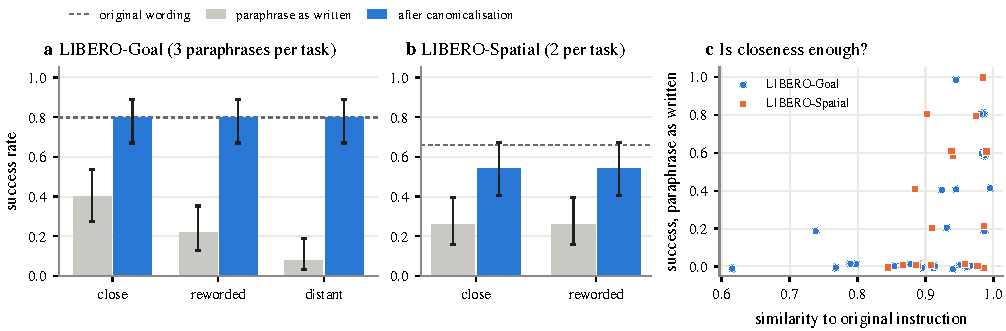
\includegraphics[width=\textwidth]{figures/language_canonical.pdf}
  \caption{\textbf{Repairing paraphrases at the input.} (a,b)~Success of hand-written paraphrases as written
  and after mapping them to the closest LIBERO training instruction, on the same episodes (5 per task and
  paraphrase); dashed: original wording. (c)~Success of each paraphrase as written against its embedding
  similarity to the original instruction.}
  \label{fig:canon}
\end{figure*}

\subsection{Repairing it at the input}
If the model only recognises training wordings, a paraphrase can be repaired before it reaches the policy.
We embed the instruction with a small sentence encoder (all-MiniLM-L6-v2,~\citep{reimers2019sbert,wang2020minilm})
and replace it by the most similar of the 40 LIBERO training instructions; below a cosine similarity of
\CanonThreshold{}, fixed before any experiment, the instruction is left unchanged. On LIBERO-Goal every
paraphrase is mapped to the right task (\RetrievalGoal{}) and success goes from \CanonGoalRaw{} to
\CanonGoal{}, the level of the original wording (\cref{fig:canon}a); the episodes are in fact identical to the
original ones, step for step. \emph{``Sing a song''} has a similarity of \AbsurdSim{} and is rejected. LIBERO-Spatial
is harder: its ten instructions differ only by where the bowl is (\emph{next to} or \emph{on} the ramekin), and
the encoder confuses 5 of 20 paraphrases (\RetrievalSpatial{} correct). Success rises from \CanonSpatialRaw{} to
\CanonSpatial{}, against \CanonSpatialRef{} with the original wording; the wrongly mapped paraphrases make the
robot execute another task. Embedding similarity predicts the success of raw paraphrases only moderately
(Spearman $\rho=\SimRho$, \cref{fig:canon}c): many paraphrases above 0.9 fail completely, so closeness in
meaning is not enough for the policy, while a lookup of known wordings is.

% =====================================================================================
\section{How does it break?}
\begin{figure*}[t]
  \centering
  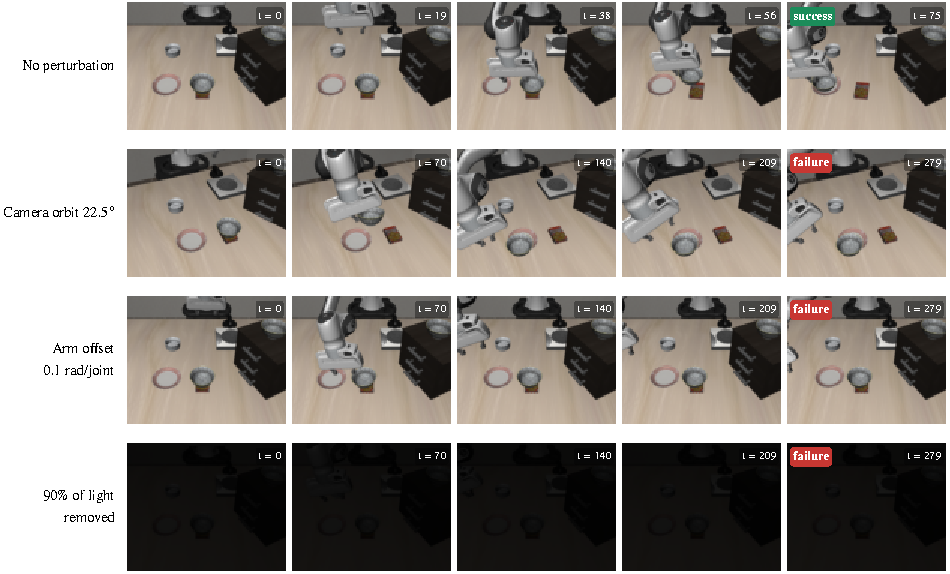
\includegraphics[width=0.8\textwidth]{figures/keyframes_failures.pdf}
  \caption{\textbf{How failures unfold} (LIBERO-Spatial task 3, initial state 2, same seed in every row).
  Under the camera orbit the bowl is picked up but ends next to the plate; with the arm offset the bowl
  is never grasped and the gripper drifts out of view; in the dark the bowl is never grasped either.}
  \label{fig:keyfail}
\end{figure*}
\label{sec:dose}
\subsection{Graded perturbations}
\begin{figure}[t]
  \centering
  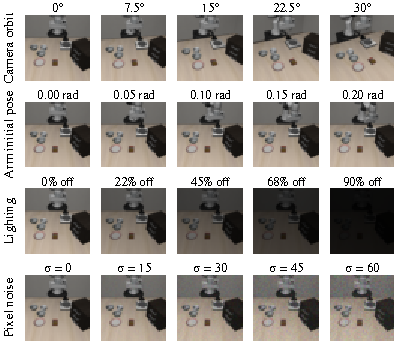
\includegraphics[width=\columnwidth]{figures/perturbation_grid.pdf}
  \caption{\textbf{Policy input at intensities} 0, 0.25, 0.5, 0.75 and 1 (LIBERO-Spatial task 0, initial
  state 0; camera shown up to $30^\circ$).}
  \label{fig:grid}
\end{figure}

Each perturbation maps an intensity $\lambda\in[0,1]$ linearly to a physical magnitude $m=\lambda\,m_{\max}$
(\cref{fig:grid}).
\begin{itemize}
  \item \textbf{Camera orbit} ($m_{\max}=60^\circ$). The agentview camera's optical axis is intersected
  with the table plane at $\bm c$; position and orientation are rotated by $R_z(\pm m)$ about the vertical
  axis through $\bm c$, so the camera keeps looking at the same point. The sign alternates with the episode.
  The wrist camera is untouched.
  \item \textbf{Arm initial pose} ($m_{\max}=0.2$\,rad). After reset, each of the seven joints is shifted by
  $s_k m$ with signs $s_k\in\{\pm1\}$ drawn once per episode, followed by five settling steps. Objects do not
  move.
  \item \textbf{Lighting} ($m_{\max}=0.9$). Diffuse, ambient and specular components of both scene lights
  and of the headlight are multiplied by $1-m$.
  \item \textbf{Pixel noise} ($m_{\max}=60$). Gaussian noise of standard deviation $m$ (0--255 scale) on both
  camera images, with a fixed seed per episode.
  \item \textbf{Camera masking}: one of the two images is replaced by black.
\end{itemize}
Simulator-level changes are re-applied after every reset, since a hard reset rebuilds the model; with soft
resets (used for RL training) the original values are cached so that changes do not compound. At the
largest intensity all task-relevant objects remain visible, except at 90\% light removal where the scene is
very dark but still readable.



\subsection{Results}


\begin{table}[t]
\centering
\caption{\textbf{Breaking points}, with 95\% task-bootstrap intervals. Levels include the unperturbed one.}
\label{tab:bp}
\scriptsize
\setlength{\tabcolsep}{3pt}
\resizebox{\columnwidth}{!}{% generated by scripts/make_tables.py -- do not edit
\begin{tabular}{llcccl}
\toprule
Perturbation & Unit & Levels & Logistic $x_{50}$ & Model-free $x_{50}$ & Shape \\
\midrule
Camera orbit & deg & 9 (0--60) & 39.7 [24.7, 61.2] & 39.4 [15, $>$60] & gradual \\
Arm initial pose & rad/joint & 8 (0--0.2) & 0.0782 [0.0504, 0.109] & 0.0477 [0.0305, 0.0821] & tolerance, then cliff \\
Lighting & fraction removed & 9 (0--0.9) & 0.761 [0.724, 0.809] & 0.744 [0.716, 0.782] & threshold \\
Pixel noise & std (0--255) & 5 (0--60) & 42.3 [35.8, 45.8] & 41.7 [34.9, 47.2] & threshold \\
\bottomrule
\end{tabular}
}
\end{table}

The curves have different \emph{shapes}, not just different scales (\cref{fig:dose}, top; \cref{tab:bp}):
\begin{itemize}
  \item \textbf{Camera orbit: gradual.} Success declines steadily with no plateau and no cliff, is halved
  around $\CamXfifty^\circ$ and remains above zero at $60^\circ$. The two orbit directions are not equally
  harmful at intermediate angles, but direction is confounded with the initial state (it alternates with
  the episode index), so we do not interpret this.
  \item \textbf{Arm initial pose: narrow tolerance, then a cliff.} Offsets up to 0.02\,rad per joint
  ($\approx1^\circ$) leave success unchanged; it is halved by $\RobotXfiftyInterp$\,rad \RobotXfiftyInterpCI{}
  (model-free; the logistic, which cannot follow both the cliff and the long tail, gives \RobotXfifty{}),
  although the objects have not moved and both cameras still see them.
  \item \textbf{Lighting: threshold.} No measurable effect up to \LightCliffLow{} of the light removed;
  success is then halved at $\LightXfiftyInterp$ and falls below a quarter of the baseline at \LightCliffHigh{}.
  \item \textbf{Pixel noise: threshold.} No effect at a standard deviation of 15, a small one at 30, halved
  at $\NoiseXfiftyInterp$ \NoiseXfiftyInterpCI{} and near zero at 60, a level at which a human still sees
  every object (\cref{fig:grid}).
\end{itemize}



\paragraph{Per-task heterogeneity} The bottom row of \cref{fig:dose} shows what the pooled curves average over. The
photometric thresholds are shared: for lighting all tasks fail between the same two levels. The viewpoint
curve is the opposite: some tasks (0 and 2) are unaffected even at $60^\circ$ while others (7 and 9) fail from
the first levels, so the pooled ``gradual'' decline is in part a mixture of task-specific cliffs. The arm
curve mixes both, with most tasks holding up to 0.03\,rad and dropping together.

\paragraph{Both cameras are needed} Blacking out one stream entirely drops success from \CamMaskBoth{} to
\CamMaskAgent{} without the third-person view and \CamMaskWrist{} without the wrist view. The policy
cannot do without the third-person image, yet tolerates rotating it by $20$--$30^\circ$ with a moderate loss,
which suggests it relies on the coarse layout of that view rather than on precise image coordinates.



\paragraph{What failures look like} \Cref{fig:keyfail} follows one episode under each perturbation. The
failures are not random motions: under the camera rotation the policy carries out the whole
pick-and-place but puts the bowl down next to the plate, as if its estimate of the plate position were
shifted; with the arm offset it never grasps the bowl and the gripper ends up out of view.

\begin{figure*}[t]
  \centering
  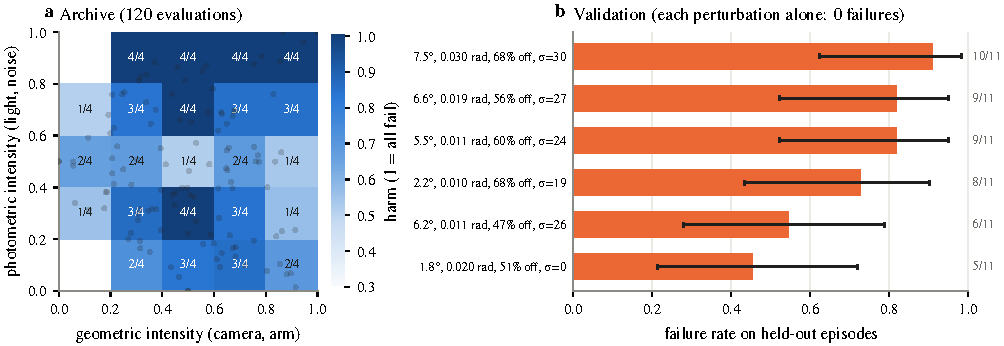
\includegraphics[width=\textwidth]{figures/qd_search.pdf}
  \caption{\textbf{Harmless alone, harmful together.} (a)~MAP-Elites archive over combinations of camera orbit
  ($\le7.5^\circ$), arm offset ($\le0.03$\,rad), light removed ($\le67.5\%$) and pixel noise ($\sigma\le30$);
  each cell shows the most harmful combination found and how many of the 4 search episodes it fails.
  Dots: all evaluated combinations. (b)~The most harmful combinations re-run on 11 held-out episodes. Dark:
  pure interactions, where each component alone at the same value succeeds on that episode; light: a
  component alone already fails.}
  \label{fig:qd}
\end{figure*}

\subsection{Harmless alone, harmful together}
The curves above vary one factor at a time. To test whether factors interact, we restrict each perturbation to
a range in which, alone, it costs at most about 15\% of the baseline (camera $\le7.5^\circ$, arm
$\le0.03$\,rad, light removed $\le67.5\%$, noise $\sigma\le30$), and select the 15 LIBERO-Spatial episodes that
succeed unperturbed \emph{and} under each of the four perturbations alone at the top of its range.

\paragraph{Search} A genome $\bm g\in[0,1]^4$ sets the four intensities. Fitness is the mean over four of these
episodes (four tasks) of 1 for a failure and $T/280$ for a success in $T$ steps, so slower successes still
guide the search; since simulation and policy are deterministic, fitness is a deterministic function of
$\bm g$. It is not a smooth one: on a given episode the outcome is not monotonic in the intensity (one
search episode fails with 51\% of the light removed but succeeds with 67.5\%), and changing a genome in the
fourth decimal can flip an episode. MAP-Elites keeps the most harmful genome in each cell of a $5\times5$ grid over geometric
(camera, arm) and photometric (light, noise) intensity. We evaluate the four single-perturbation maxima and
the full combination, 15 random genomes, then Gaussian mutations ($\sigma=0.15$) of random elites, for
\QDEvals{} evaluations (\QDEpisodes{} episodes). The six most harmful elites are then re-run on the 11 remaining
episodes. Because of the non-monotonicity, checking each perturbation alone at the top of its range does not
rule out that it fails alone at an intermediate value. As a control, every component of every validated
combination is also run alone, at the same value, on the same held-out episodes (\QDControlEpisodes{}
episodes); a failure counts as a \emph{pure interaction} only if every component alone succeeds on that episode.

\paragraph{Results} As designed, the single-perturbation maxima fail \QDSingleFails{} search episodes; their
combination fails \QDCornerFails{}. Failures are not confined to that corner: \QDAnyFail{} evaluated combinations
fail at least one episode and all \QDFailCells{} filled cells contain one (\cref{fig:qd}a). The most harmful
elites transfer to the held-out episodes, where they produce \QDValPooled{} failures (\cref{fig:qd}b). The
single-component controls fail \QDControlFails{} episodes, mostly the camera orbit at intermediate angles,
so \QDSingleAlsoFail{} of these failures are not pure interactions; the remaining \QDPure{} are. The full
combination fails \QDValCorner{} held-out episodes, all pure interactions, and even the smallest elite
($1.8^\circ$, 0.02\,rad, half of the light removed, no noise) fails 5 of 11, 3 of them pure.
Across the evaluated combinations, harm correlates most with pixel noise (Spearman $\rho=\QDRhoNoise$) and
arm offset ($\rho=\QDRhoArm$), and little with camera angle ($\QDRhoCam$) or lighting ($\QDRhoLight$) within
these ranges; the search does not sample uniformly, so these correlations are only indicative. Robustness measured
one factor at a time therefore overestimates the margin available when several conditions drift together.

% =====================================================================================
\section{Can a small corrector fix it?}
\begin{figure*}[t]
  \centering
  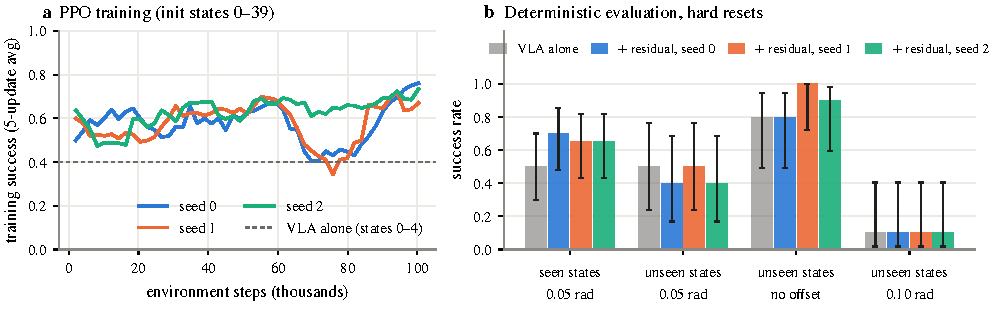
\includegraphics[width=\textwidth]{figures/rl_residual.pdf}
  \caption{\textbf{Residual RL on the arm-offset weakness.} (a)~Success of the stochastic policy during PPO,
  moving average over 5 updates; dashed: runs trained with new random offset signs at every reset.
  (b)~Deterministic evaluation with hard resets on initial states seen in training (0--19) and held out
  (40--49). Wilson 95\% intervals.}
  \label{fig:rl}
\end{figure*}
\label{sec:rl}
\subsection{Residual RL formulation}
We target the arm-pose weakness, which is the one visible in proprioception: a corrector without images
can in principle detect it. The task is LIBERO-Spatial task 2 at 0.05\,rad per joint, where the VLA alone
succeeds in about half of the episodes. At step $t$ the corrector observes
$\bm o_t=(\bm p_t,\bm q_t,\bm g_t,\bm a^{\mathrm{VLA}}_t,t/T)\in\mathbb{R}^{17}$ (end-effector position and
quaternion, gripper opening, the VLA's action for this step, progress) and outputs
$\Delta\bm a_t\in[-1,1]^7$; the executed action is
\begin{equation}
  \bm a_t=\mathrm{clip}\big(\bm a^{\mathrm{VLA}}_t+\alpha\,\Delta\bm a_t,\,-1,\,1\big),\qquad \alpha=0.2 .
\end{equation}
The reward is 1 on success and 0 otherwise; episodes end on success or after $T=280$ steps. Actor and critic
are separate MLPs (\cref{tab:ppo}); the actor's last layer is initialised to zero, so before training the
corrected policy \emph{is} the VLA, which we verified on full episodes (identical outcomes and episode
lengths). We train with PPO~\citep{schulman2017ppo} in a single-file implementation in the style of
CleanRL~\citep{huang2022cleanrl}, four simulators in one process sharing batched VLA queries (about 10
steps/s), soft resets during training, and 100k environment steps per run (about 400 episodes). Initial
states 0--39 are used for training; 40--49 are held out. Evaluation uses the deterministic mean action and
hard resets, like every other number in this report.



\begin{table}[t]
\centering
\caption{\textbf{Residual RL evaluation} (successes / episodes, offset in rad per joint). ``Re-plan / 10''
executes 10 instead of 50 actions per chunk, without any learning. s0--s2: residual seeds with fixed
offset signs per initial state; rs0--rs1: trained with new random signs at every reset.}
\label{tab:rl}
\scriptsize
\setlength{\tabcolsep}{3pt}
\resizebox{\columnwidth}{!}{% generated by scripts/make_tables.py -- do not edit
\begin{tabular}{llcccc}
\toprule
Initial states & Offset (rad) & VLA & + res. s0 & + res. s1 & Re-plan / 10 \\
\midrule
Seen (0--19) & 0.05 & 10/20 & 14/20 & 13/20 & -- \\
Held-out (40--49) & 0.05 & 5/10 & 4/10 & 5/10 & 4/10 \\
Held-out (40--49) & 0 & 8/10 & 8/10 & 10/10 & 10/10 \\
Held-out (40--49) & 0.10 & 1/10 & 1/10 & 1/10 & 3/10 \\
\midrule
\multicolumn{2}{l}{Seen: steps per success} & 110 & 91 & 90 & \\
\multicolumn{2}{l}{Seen: McNemar $p$ vs VLA} & & 0.12 & 0.38 & \\
\multicolumn{2}{l}{Held-out: steps per success} & 95 & 89 & 92 & \\
\multicolumn{2}{l}{Held-out: McNemar $p$ vs VLA} & & 1.00 & 1.00 & \\
\bottomrule
\end{tabular}
}
\end{table}

\subsection{Results}
Training success rises modestly (from \RLTrainFirst{} to \RLTrainLast{} over the first and last ten updates
of each of the \SeedsWord{} seeds; \cref{fig:rl}a), and two of the three runs dip around 70k steps before
recovering. On initial states seen in training, the deterministic
corrector succeeds in \RLSeenRes{} episodes against \RLSeenVla{} for the VLA alone, and every discordant
episode favours the corrector (\cref{tab:rl}; McNemar $p=$ \RLPSeen{}, not significant at this sample
size). On held-out initial states the gain disappears: \RLUnseenRes{} against \RLUnseenVla{} at the training
level and \RLUnseenStrongRes{} against \RLUnseenStrongVla{} at 0.10\,rad. The corrector does not hurt the
unperturbed task (\RLUnseenCleanRes{} against \RLUnseenCleanVla{}).

\paragraph{What is learned} What transfers is speed: successful episodes are shorter with the corrector,
from \RLStepsSeenVla{} to \RLStepsSeenRes{} steps on seen states and from \RLStepsUnseenVla{} to
\RLStepsUnseenRes{} on held-out ones. This is what the objective rewards most directly: with discounting a
faster success is worth more, and an episode that already works can be sped up in every rollout, whereas
recovering a failure is a rare event in 400 episodes. The recoveries that do occur are tied to the
configurations seen in training; with 40 of them, a proprioceptive corrector has little to interpolate from.

\paragraph{More diverse starts do not help} If the corrector fails to generalise because it only saw 40
offset patterns (signs are tied to the initial state), drawing new signs at every training reset should
help. It does not: with random signs, the corrector reaches \RLRandSeenRes{} on the seen initial states and
\RLRandUnseenRes{} on held-out ones at the training level (against \RLSeenVla{} and \RLUnseenVla{} for the VLA
alone), the same pattern as before. The bottleneck is therefore not the variety of arm offsets but the
variety of scenes, or what a proprioceptive corrector can infer about them.

\paragraph{A training-free alternative} Executing 10 instead of 50 actions per chunk, so that the VLA
re-plans five times more often, gives \RLReplanClean{}, \RLReplanTrain{} and \RLReplanStrong{} on the
held-out episodes (no offset, 0.05 and 0.10\,rad), not distinguishable from the VLA alone with 10 episodes, at
\RLReplanSlowdown{}$\times$ the cost.

% =====================================================================================
\section{Limitations and threats to validity}
\begin{itemize}
  \item \textbf{Scope.} One model, one checkpoint, two LIBERO suites, simulation only. The measured
  baselines are below published numbers; we report changes relative to them.
  \item \textbf{Sample size.} 3--10 episodes per cell. Intervals are wide and many per-task differences are
  within noise; we report intervals rather than significance stars and do not correct for multiple
  comparisons.
  \item \textbf{Shared episodes.} Using the same initial states and seeds across conditions removes noise
  from comparisons but correlates them: a hard initial state is hard in every condition.
  \item \textbf{Numerics.} Inference ran on Apple's Metal backend in bf16; results on CUDA may differ slightly.
  A GPU runner with the same configurations is provided but was not used for reported numbers.
  \item \textbf{Paraphrases} were written by one person and are not a sample of how users phrase tasks.
  \item \textbf{Camera direction} is confounded with the initial state; we only interpret magnitude.
  \item \textbf{Canonicalisation} needs the list of known tasks and cannot help with a genuinely new
  instruction; its encoder loses spatial relations.
  \item \textbf{Failure search} used four episodes for fitness, so elites can overfit them; the held-out
  validation (11 episodes) limits but does not remove this. Episode outcomes are not monotonic in the
  intensity, which is why interactions are only counted against single-component controls at the same
  values. The archive descriptors are one choice among many.
  \item \textbf{Residual RL} used one task, one perturbation level, about 400 training episodes per run and
  soft resets during training, so its negative result says more about this budget than about residual RL.
\end{itemize}

% =====================================================================================
\section{Conclusion}
On LIBERO, SmolVLA is neither deaf to language nor robust to it: the instruction decides which task is
attempted, but only in wordings close to those seen in training, and a simple lookup of known wordings
repairs most paraphrases. Its failures under distribution shift have distinct shapes, gradual for
viewpoint and abrupt for lighting, noise and arm configuration, and perturbations that are harmless one at a
time become harmful together, which one-factor-at-a-time benchmarks cannot reveal. \RLRandConclusion{}
Natural next steps are the same protocol on larger VLAs and a search over a richer space of scene changes.

\paragraph{Reproducibility} Every number in this report is generated from the per-episode CSV files by
scripts in the repository, which also contains the configurations, the trained correctors and the
rollout videos.

{\small
\bibliographystyle{abbrvnat}
\setlength{\bibsep}{1.5pt}
\bibliography{refs}
}

% =====================================================================================
\appendix
\section{Additional tables}
\begin{table}[h]
\centering
\caption{\textbf{Unperturbed successes per task} (out of 10).}
\label{tab:pertask}
\scriptsize
\setlength{\tabcolsep}{3pt}
% generated by scripts/make_tables.py -- do not edit
\begin{tabular}{lccccccccccc}
\toprule
Task & 0 & 1 & 2 & 3 & 4 & 5 & 6 & 7 & 8 & 9 & All \\
\midrule
Spatial & 10 & 6 & 7 & 6 & 4 & 1 & 8 & 8 & 2 & 7 & 59/100 \\
Goal & 10 & 10 & 9 & 8 & 8 & 8 & 4 & 9 & 8 & 10 & 84/100 \\
\bottomrule
\end{tabular}

\end{table}

\begin{table}[h]
\centering
\caption{\textbf{PPO configuration}, read from the saved checkpoints.}
\label{tab:ppo}
\scriptsize
% generated by scripts/make_tables.py -- do not edit
\begin{tabular}{ll}
\toprule
Task / perturbation & Spatial task 2, arm offset 0.05 rad/joint \\
Correction scale $\alpha$ & 0.2 \\
Policy / value network & MLP, 2 $\times$ 128 tanh, separate \\
Initial std of $\Delta a$ & $e^{-1}$ \\
Parallel environments & 4 \\
Steps per env per rollout & 512 \\
Total environment steps & 100\,000 \\
Epochs / minibatch & 10 / 256 \\
Learning rate (Adam) & 0.0003 \\
$\gamma$ / GAE $\lambda$ & 0.995 / 0.95 \\
Clip / value coef. / entropy coef. & 0.2 / 0.5 / 0.0 \\
Max grad norm & 0.5 \\
VLA actions per chunk executed & 50 \\
Training init states & 0--39 \\
\bottomrule
\end{tabular}

\end{table}

\begin{table}[h]
\centering
\caption{\textbf{Compute.} Wall-clock time on an Apple M1 laptop (8\,GB), one process at a time.}
\label{tab:compute}
\scriptsize
% generated by scripts/make_tables.py -- do not edit
\begin{tabular}{lrrr}
\toprule
Experiment & Episodes & s / episode & Hours \\
\midrule
Baselines & 200 & 29 & 1.6 \\
Listening matrix & 300 & 26 & 2.2 \\
Instruction variants & 250 & 37 & 2.6 \\
Dose-response (4 families) & 1350 & 27 & 10.2 \\
Camera masking & 100 & 31 & 0.9 \\
Instruction canonicalisation & 350 & 18 & 1.8 \\
Residual RL evaluation & 335 & 21 & 2.0 \\
Validation re-runs & 4 & 12 & 0.0 \\
Failure search (MAP-Elites) & 799 & 21 & 4.6 \\
PPO training (5 runs) & -- & -- & 14.4 \\
\midrule
Total & 3688 & & 40.2 \\
\bottomrule
\end{tabular}

\end{table}



\end{document}
